\section{Laboratorio No 05 – Cuestionario} 

\begin{enumerate}[1.]
	\item Los valores introducidos al archivo sysctl.conf ¿que representan?	
	\\
	\\El fichero de configuración /etc/sysctl.conf se utiliza para establecer algunos parámetros del kernel y que estos se mantengan 	entre sucesivos arranques del sistema.
\\
\\fs.suid\_dumpable :
	\\El parámetro \- kernel es requerido cuando se recupera un archivo core de un proceso que cambia el USUARIO EFECTIVO LLAMANDO por sí mismo la llamada del sistema suid. Cambie también el kernel kernel.core\_pattern si lo desea. Puede cambiar los parámetros del núcleo en línea usando el comando sysctl -w, como se muestra:

 sysctl -w fs.suid\_dumpable = 1
\\
\\fs.aio-max-nr:
	\\Al instalar una base de datos Oracle en un servidor Linux, por ejemplo Ubuntu , puede encontrar una advertencia durante la instalación de que debe cambiar su parámetro aio-max-nr. Esta advertencia probablemente vendrá en un formato como el siguiente: 
Esta es una condición previa para probar si el parámetro del núcleo del sistema operativo "aio-max-nr" está configurado correctamente.
\\ 
Valor esperado: 1048576 
Valor real: 65536
\\
\\fs.file-max
\\Muchas aplicaciones, como la base de datos Oracle o el servidor web Apache, necesitan este rango bastante más alto. De modo que puede aumentar la cantidad máxima de archivos abiertos estableciendo un nuevo valor en la variable kernel / proc / sys / fs / file-max de la siguiente manera (inicie sesión como raíz): 
\\
 sysctl -w fs.file-max=100000
\\
\\kernel.shmmni:
\\Uno de los valores que afectan a oracle en el kernel de Linux. Es importante saber cómo mirar los valores del Kernel en Linux definidos para Oracle. Esto nos puede ser útil para cuando vamos a realizar una instalación del servidor de Base de datos, o bien cuando queremos modificar algún parámetro ya definido anteriormente.
\\
\\kernel.sem:
\\Para los parámetros del semáforo (kernel.sem) , debe especificar los cuatro valores.
En los sistemas SUSE Linux Enterprise Server, debe realizar otro comando para asegurarse de que el sistema lo lea.
\\
\\net.ipv4.ip\_local\_port\_range:
\\Para servidores de red de tráfico pesado, como servidores proxy o equilibradores de carga, es posible que necesite aumentar el rango de puertos de red.
En Linux, hay un parámetro sysctl llamado ip\_local\_port\_range que define el puerto mínimo y máximo que una conexión de red puede usar como su puerto de origen (local). Esto se aplica a las conexiones TCP y UDP.
\\
\\net.core.rmem\_default: 
\\El valor por default y maximo de memoria para recepcion de paquetes.
root@ascariote:~\# cat /proc/sys/net/core/rmem\_default
112640
\\
\\net.core.rmem\_max: 
\\Ajusta el máximo de bufer de recepción para todos los protocolos.
\\
\\net.core.wmem\_default: 
\\El valor por default y maximo de memoria para envio de paquetes.
root@ascariote:~\# cat /proc/sys/net/core/wmem\_default
\\
\\net.core.wmem\_max: 
\\Ajusta el máximo de bufer de envio para todos los protocolos.
\\










	
	\item ¿Con qué usuario(s) puedo conectarme al servidor a través del Administrador Empresarial?
	\\
	\\ se podra ingresar con 2 grupos de usuarios oinstall y dba, así como una cuenta de usuario llamada oracle

	\item Capture una imagen de pantalla del navegador con el Administrador Empresarial, con el nombre de su servidor e iniciada la sesión del usuario SYS.

	\begin{center}
	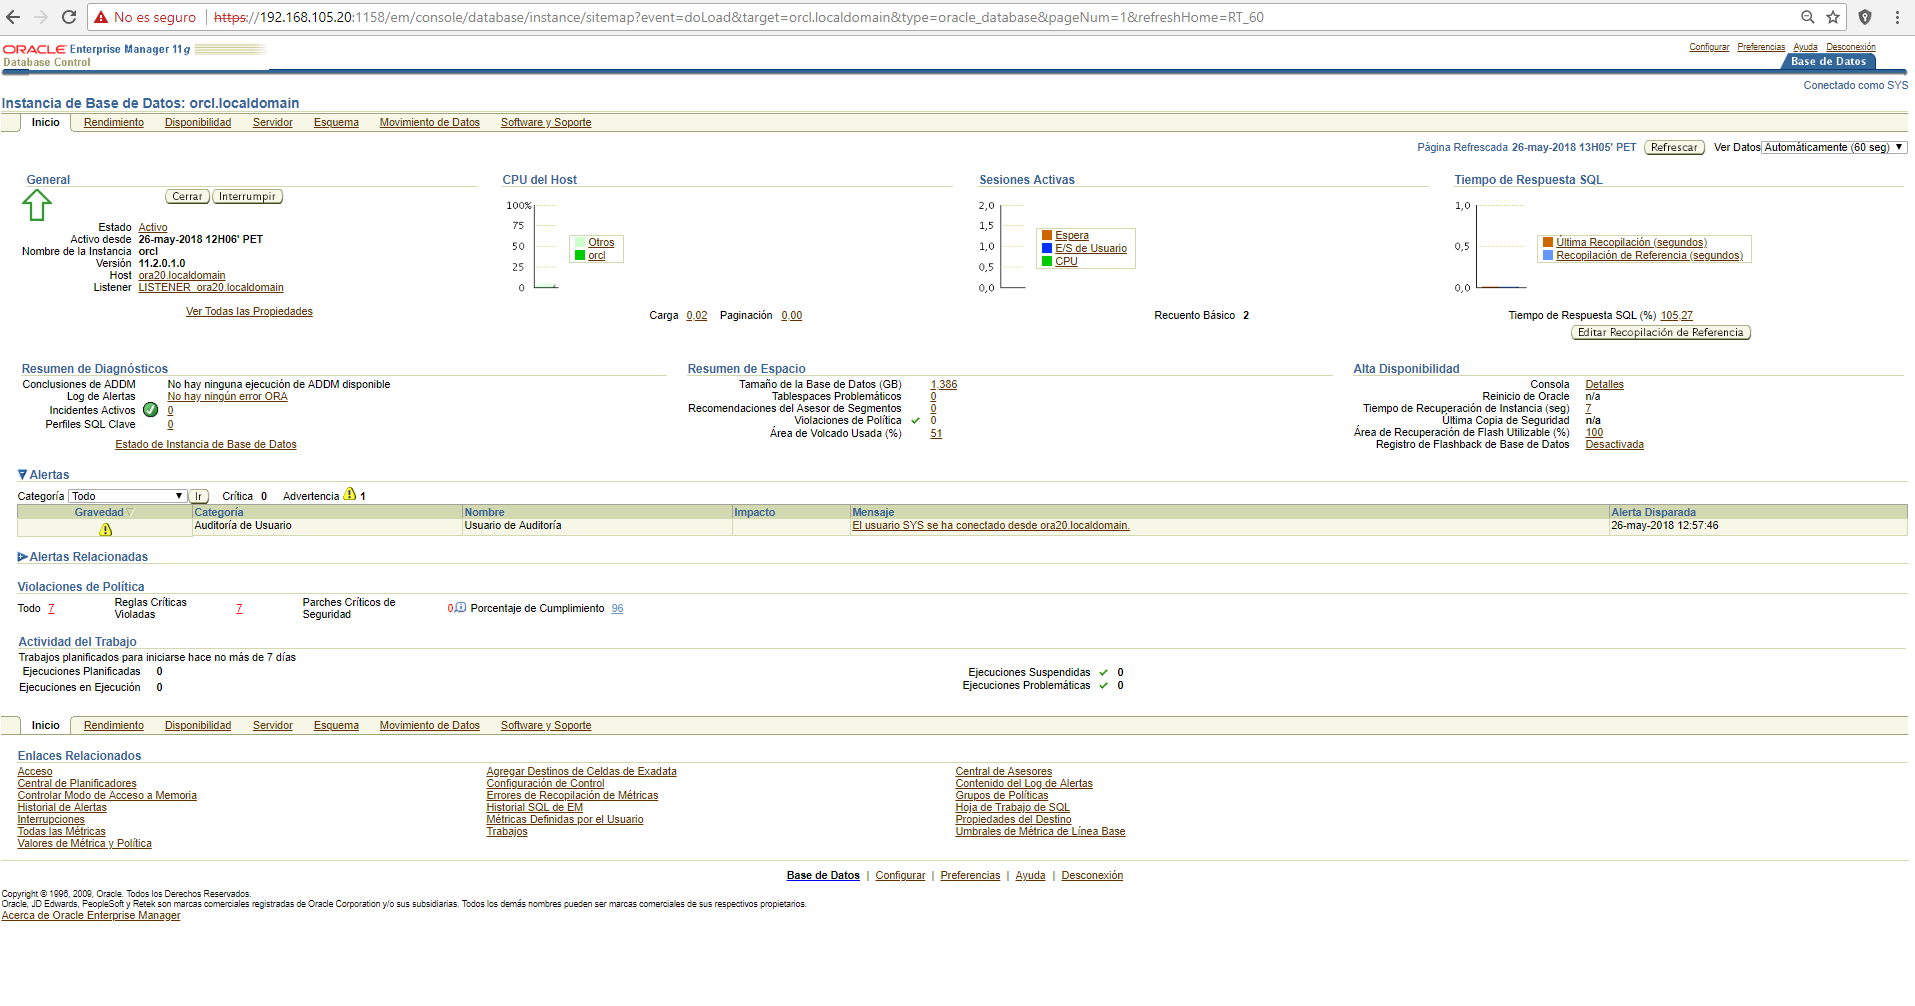
\includegraphics[width=15cm]{./Imagenes/Lab5-5_3} 
	\end{center}
	
	

\end{enumerate} 
